\documentclass[12pt]{beamer}
\newenvironment{ConCodigo}[1]
  {\begin{frame}[fragile,environment=ConCodigo]{#1}}
  {\end{frame}}
\graphicspath{{Imagenes/}{../Imagenes/}}
\usepackage[utf8]{inputenc}
\usepackage[spanish]{babel}
\usepackage{hyperref}
\usepackage{etex}
%\reserveinserts{28}
\usepackage{amsmath}
\usepackage{amsthm}
\usepackage{mathtools}
\usepackage{multicol}
\usepackage{multirow}
\usepackage{tabulary}
\usepackage{booktabs}
\usepackage{nccmath}
\usepackage{physics}
\usepackage{biblatex}
\usepackage[outdir=./]{epstopdf}
%\epstopdfsetup{outdir=./}
\usepackage{graphicx}
%\usepackage{enumitem,xcolor}
\usepackage{siunitx}
%\sisetup{scientific-notation=true}
%\usepackage{fontspec}
\usepackage{lmodern}
\usepackage{float}
\usepackage[format=hang, font=footnotesize, labelformat=parens]{caption}
\usepackage[autostyle,spanish=mexican]{csquotes}
\usepackage{standalone}
\usepackage{blkarray}
\usepackage{algorithm}
\usepackage{algorithmic}
\usepackage{tikz}
\usepackage[siunitx, RPvoltages]{circuitikz}
\usetikzlibrary{arrows,patterns,shapes}
\usetikzlibrary{decorations.markings}
\usetikzlibrary{arrows}
\usepackage{color}
\usepackage{xcolor}
%\usepackage{beton}
%\usepackage{euler}
%\usepackage[T1]{fontenc}
\usepackage[sfdefault]{roboto}  %% Option 'sfdefault' only if the base font of the document is to be sans serif
\usepackage[T1]{fontenc}
\renewcommand*\familydefault{\sfdefault}
\DeclareGraphicsExtensions{.pdf,.png,.jpg}
\usepackage{hyperref}
\renewcommand {\arraystretch}{1.5}
\newcommand{\python}{\texttt{python}}
\usefonttheme[onlymath]{serif}
\setbeamertemplate{navigation symbols}{}
\usetikzlibrary{patterns}
\usetikzlibrary{decorations.markings}
\tikzstyle{every picture}+=[remember picture,baseline]
%\tikzstyle{every node}+=[inner sep=0pt,anchor=base,
%minimum width=2.2cm,align=center,text depth=.15ex,outer sep=1.5pt]
%\tikzstyle{every path}+=[thick, rounded corners]
\setbeamertemplate{caption}[numbered]
\newcommand{\ptm}{\fontfamily{ptm}\selectfont}
%Se usa la plantilla Warsaw modificada con spruce
\mode<presentation>
{
  \usetheme{Warsaw}
  \setbeamertemplate{headline}{}
  \useoutertheme{default}
  \usecolortheme{albatross}
  \setbeamercovered{invisible}
}
% \AtBeginSection[]
% {
% \begin{frame}<beamer>{Contenido}
% \normalfont\mdseries
% \tableofcontents[currentsection]
% \end{frame}
% }

\include{pre_codigo}
\title{Tema 0 - Programaci\'{o}n b\'{a}sica con Python III}
\subtitle{Curso de F\'{i}sica Computacional}
\author[]{M. en C. Gustavo Contreras May\'{e}n}
\date{}

\begin{document}
\maketitle
\fontsize{14}{14}\selectfont
\spanishdecimal{.}
\AtBeginSection[]
{
\begin{frame}{Contenido}
\tableofcontents[ 
    currentsubsection, 
    hideothersubsections, 
    sectionstyle=show/hide, 
    subsectionstyle=show/shaded, 
    hideothersubsections
    ] 
\end{frame}
}\section{Usando gEdit}
\begin{frame}
\frametitle{Usando gEdit}
gedit es un editor de textos compatible con UTF-8 para GNU/Linux, Mac OS X y Microsoft Windows. Diseñado como un editor de textos de prop\'{o}sito general, gedit enfatiza la simplicidad y  facilidad de uso. Incluye herramientas para la edici\'{o}n de c\'{o}digo fuente y textos estructurados, como lenguajes de marcado.
\\
\medskip
Es el editor predeterminado de GNOME.
\\
\medskip
Distribuido bajo las condiciones de la licencia GPL, gedit es software libre.
\end{frame}
\begin{frame}[fragile]
\begin{figure}
	\centering
	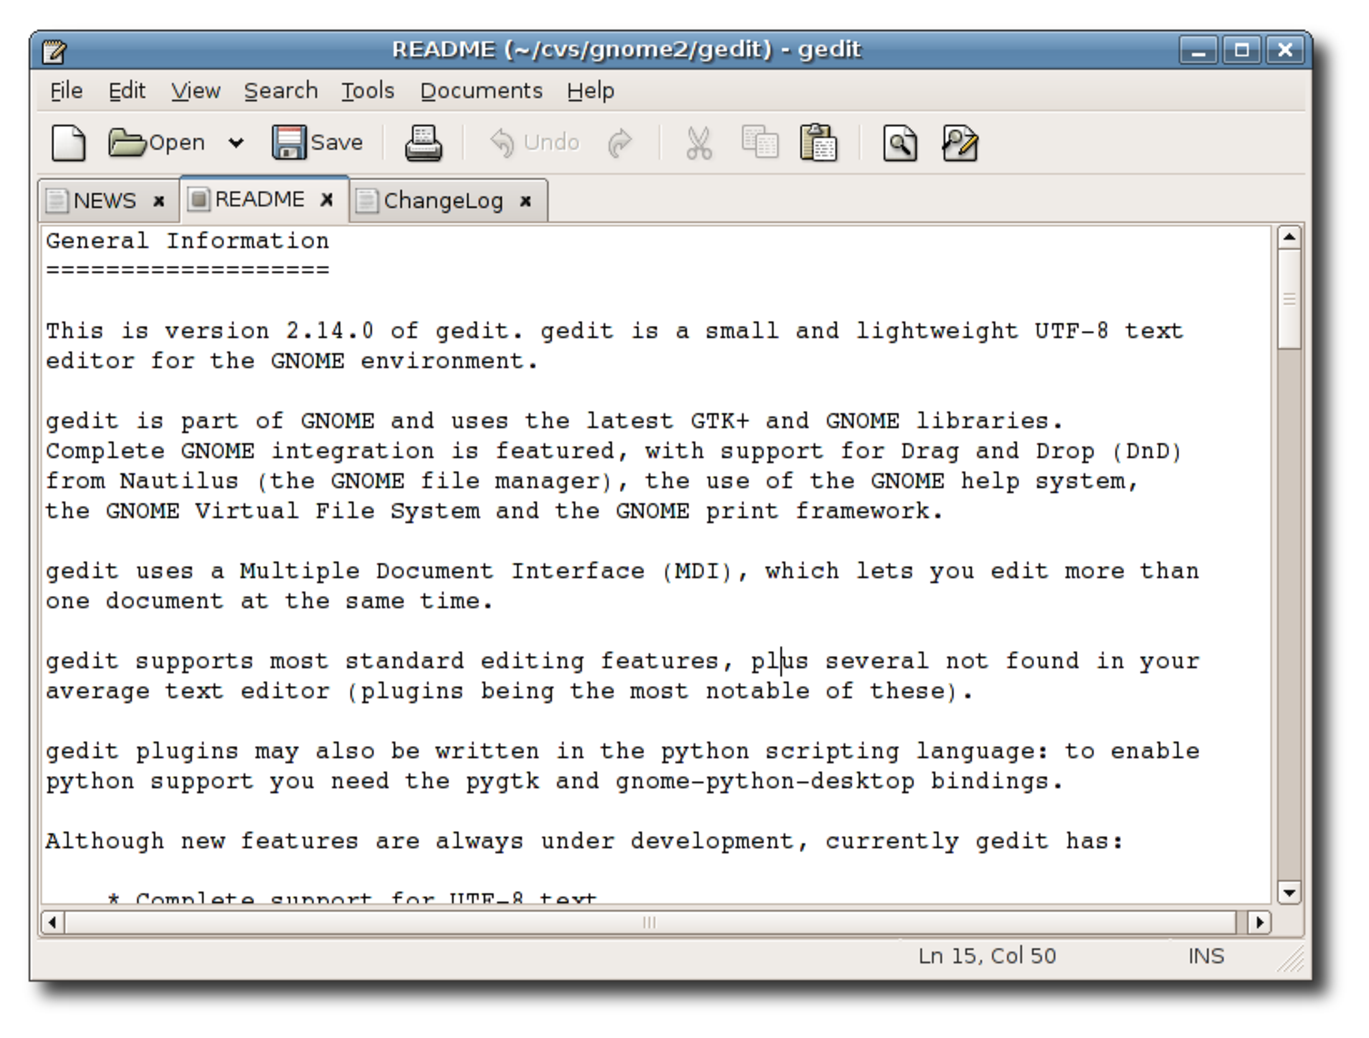
\includegraphics[scale=0.5]{gedit1.eps}<1> 
	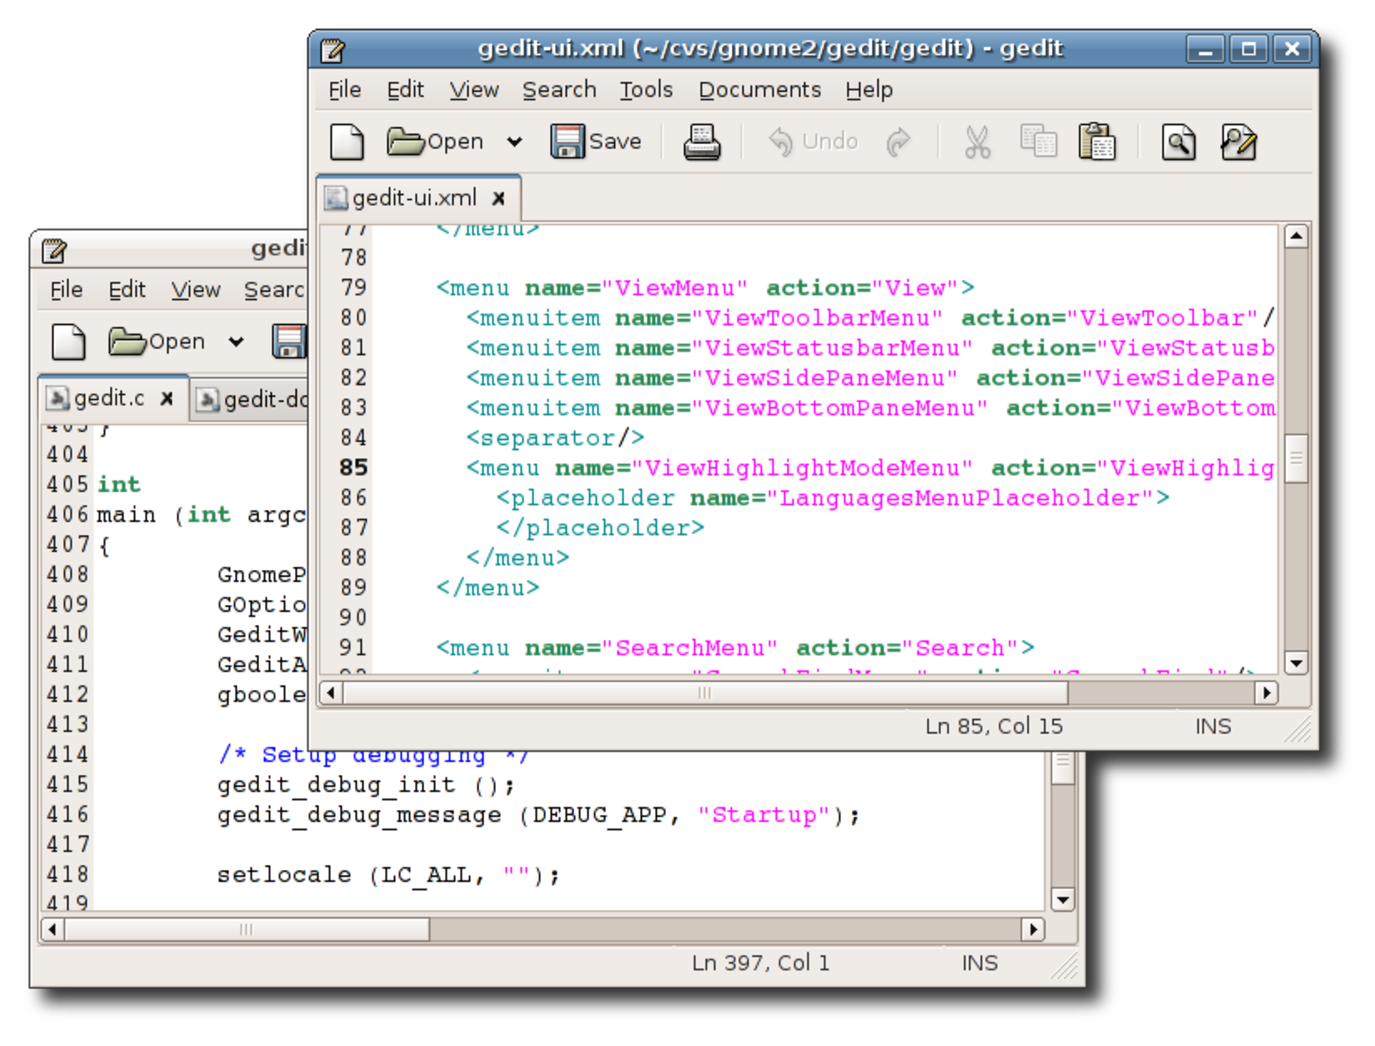
\includegraphics[scale=0.5]{gedit2.eps}<2>
	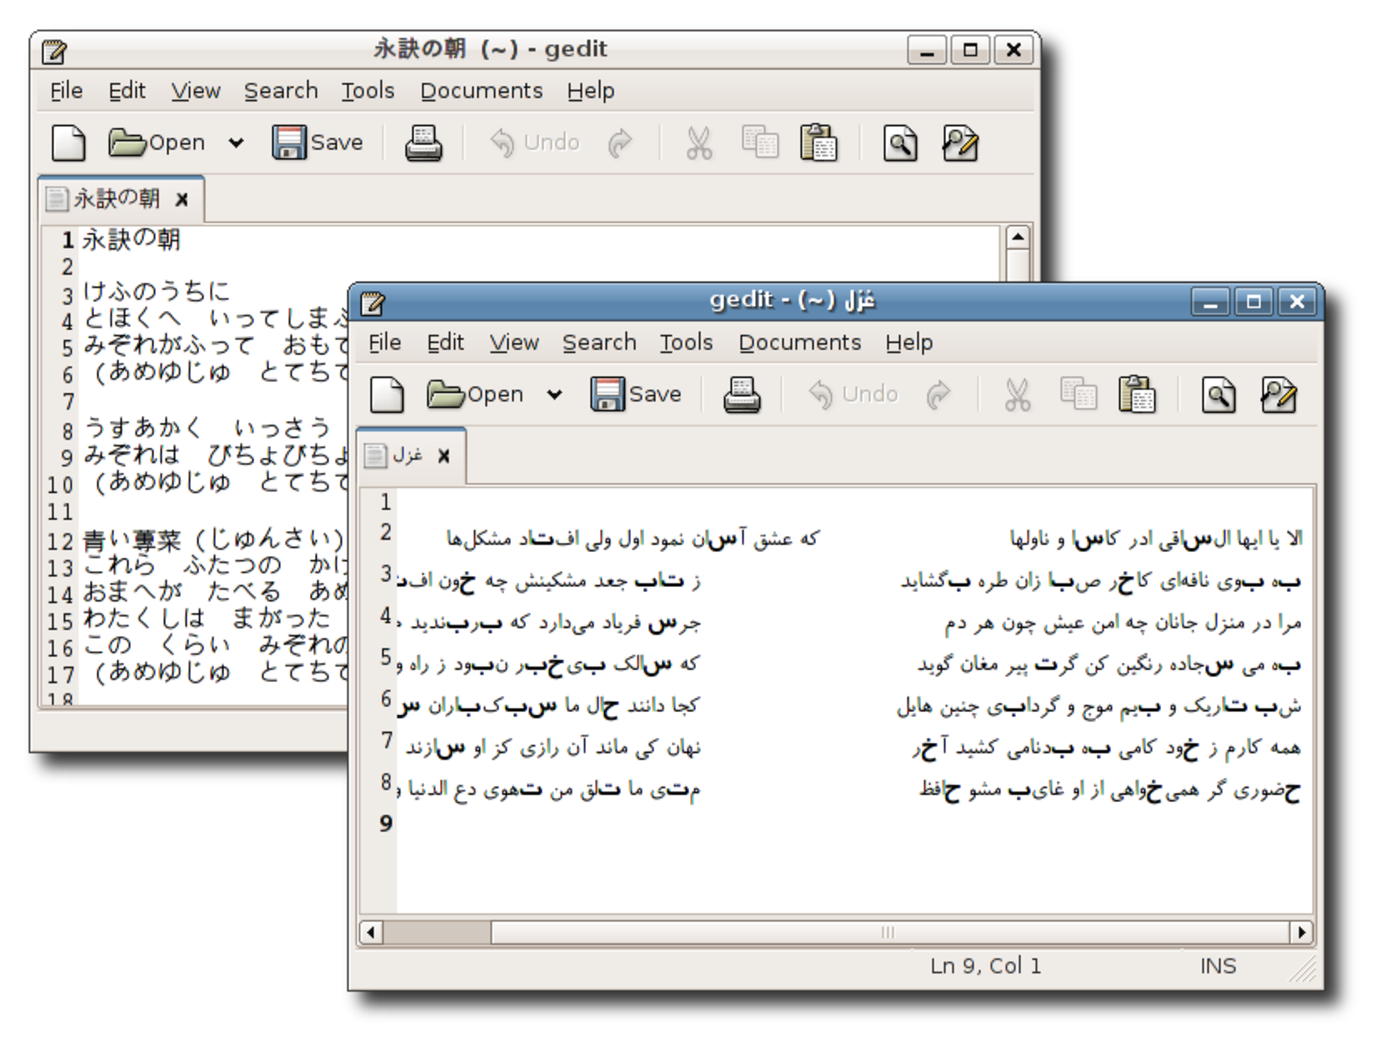
\includegraphics[scale=0.5]{gedit3.eps}<3>
	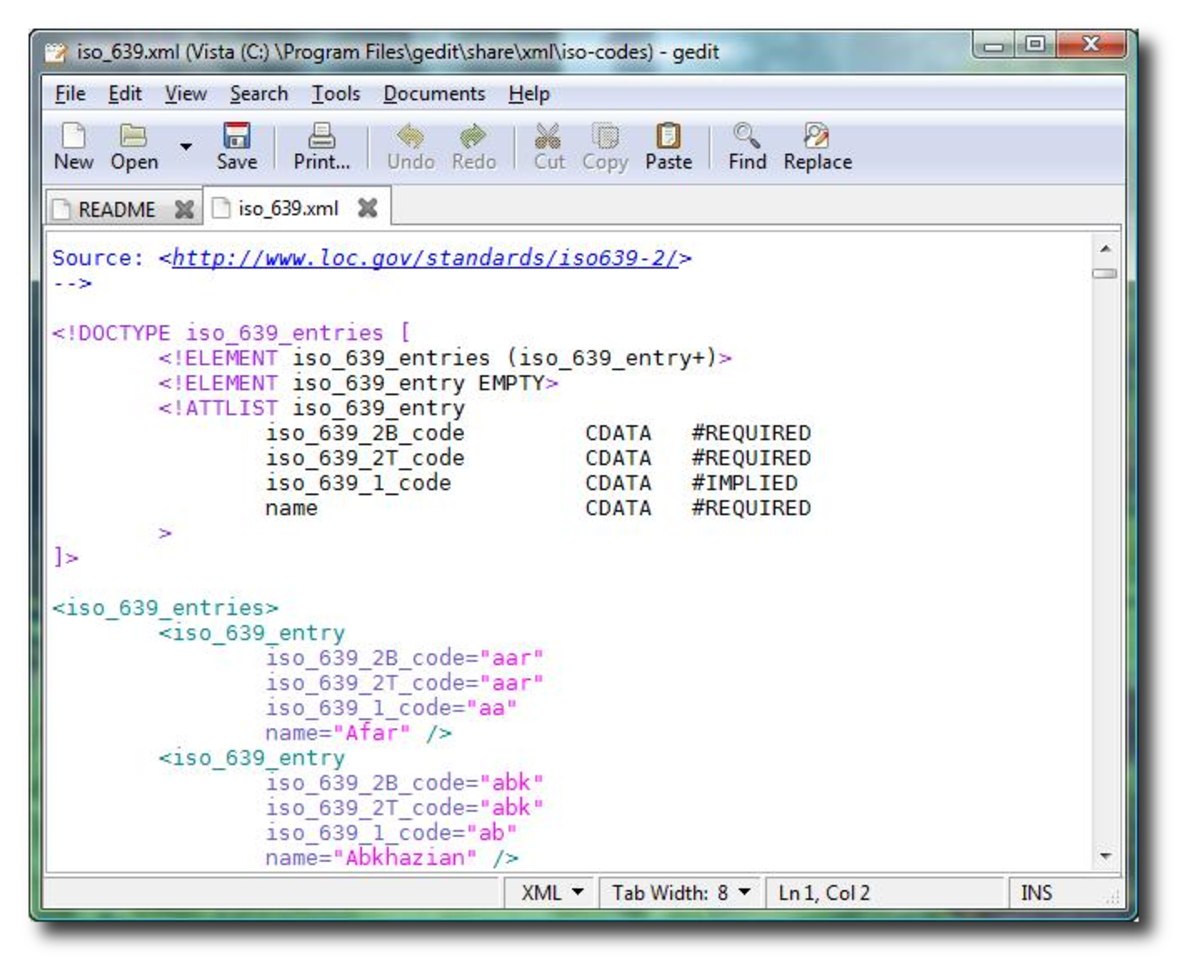
\includegraphics[scale=0.5]{gedit4.eps}<4>
	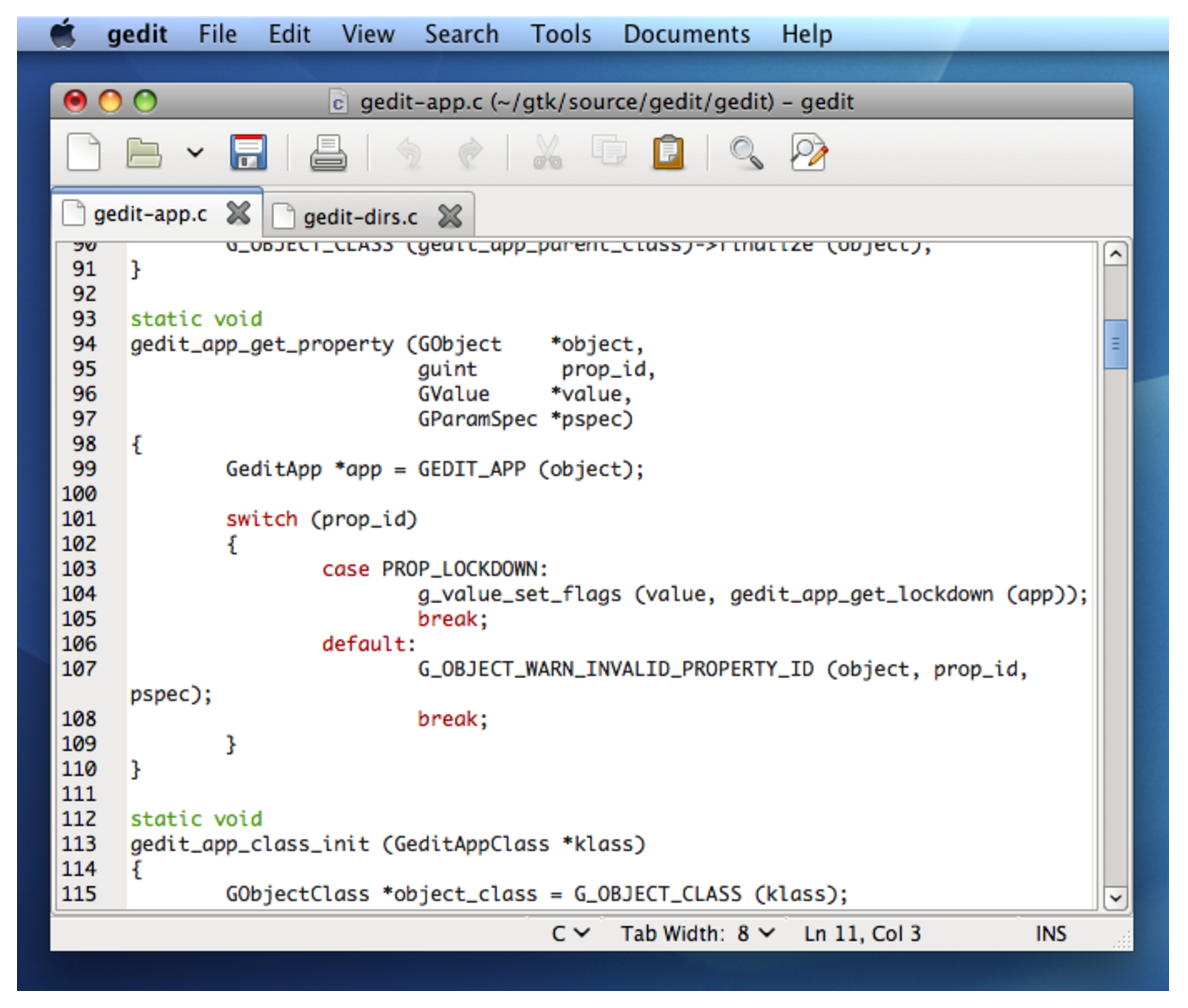
\includegraphics[scale=0.5]{gedit5.eps}<5>
\end{figure}
\end{frame}
\section{Spyder 2}
\begin{frame}
\frametitle{El entorno Spyder2}
Spyder es un entorno de desarrollo integrado para el lenguaje Python con pruebas interactivas y avanzadas funciones de depuraci\'{o}n, introspecci\'{o}n y edici\'{o}n.
\\
\medskip
Spyder permite trabajar f\'{a}cilmente con las mejores herramientas de la pila cient\'{i}fica de Python en un entorno sencillo y potente.
\end{frame}
\begin{frame}[fragile]
Estas son algunas de las caracter\'{i}sticas clave de Spyder:
\begin{enumerate}[<+->]
\item Cuadro de di\'{a}logo de administraci\'{o}n de \texttt{PYTHONPATH} como de MATLAB (funciona con todas las consolas)
\item Editor de variables de entorno de usuario actual.
\item Enlaces directos a la documentaci\'{o}n (Python, Matplotlib, NumPy, Spicy, etc.)
\item Enlace directo al lanzador de Python(x,y)
\item Enlaces directos a QtDesigner, QtLinguist y QtAssistant (documentación de Qt)
\end{enumerate}
\end{frame}
\begin{frame}
\begin{figure}
	\centering
	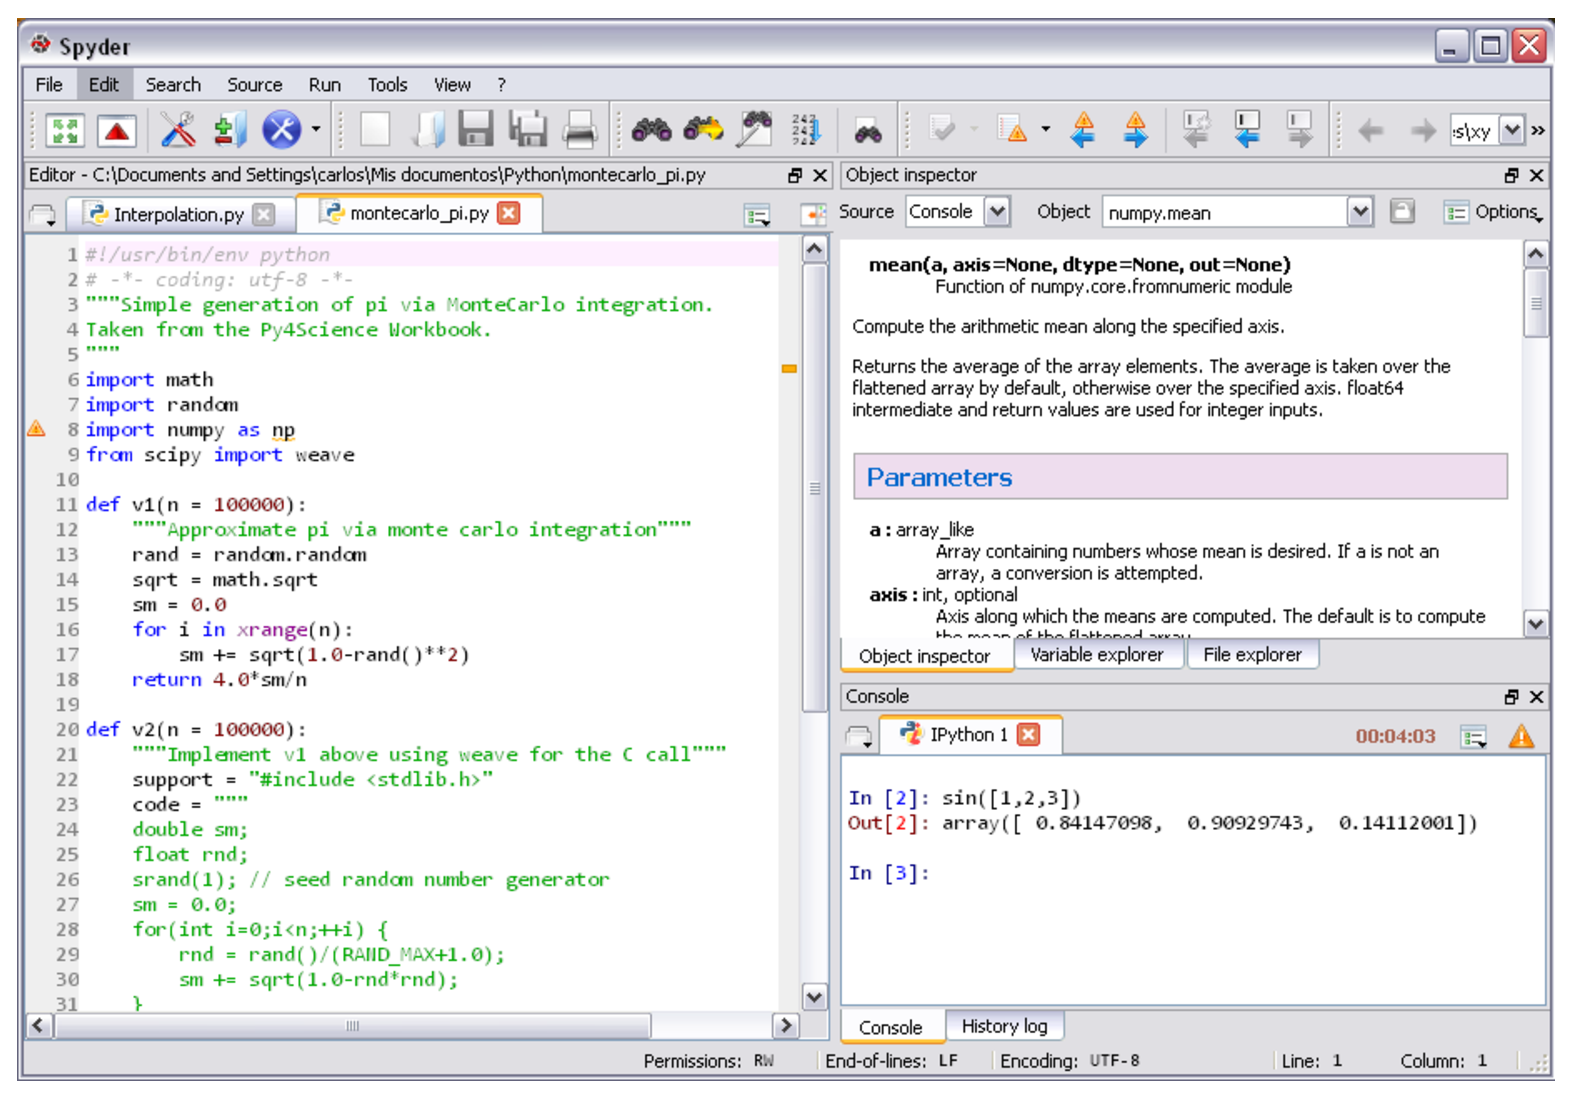
\includegraphics[scale=0.5]{spyder-windows.eps}<1>
	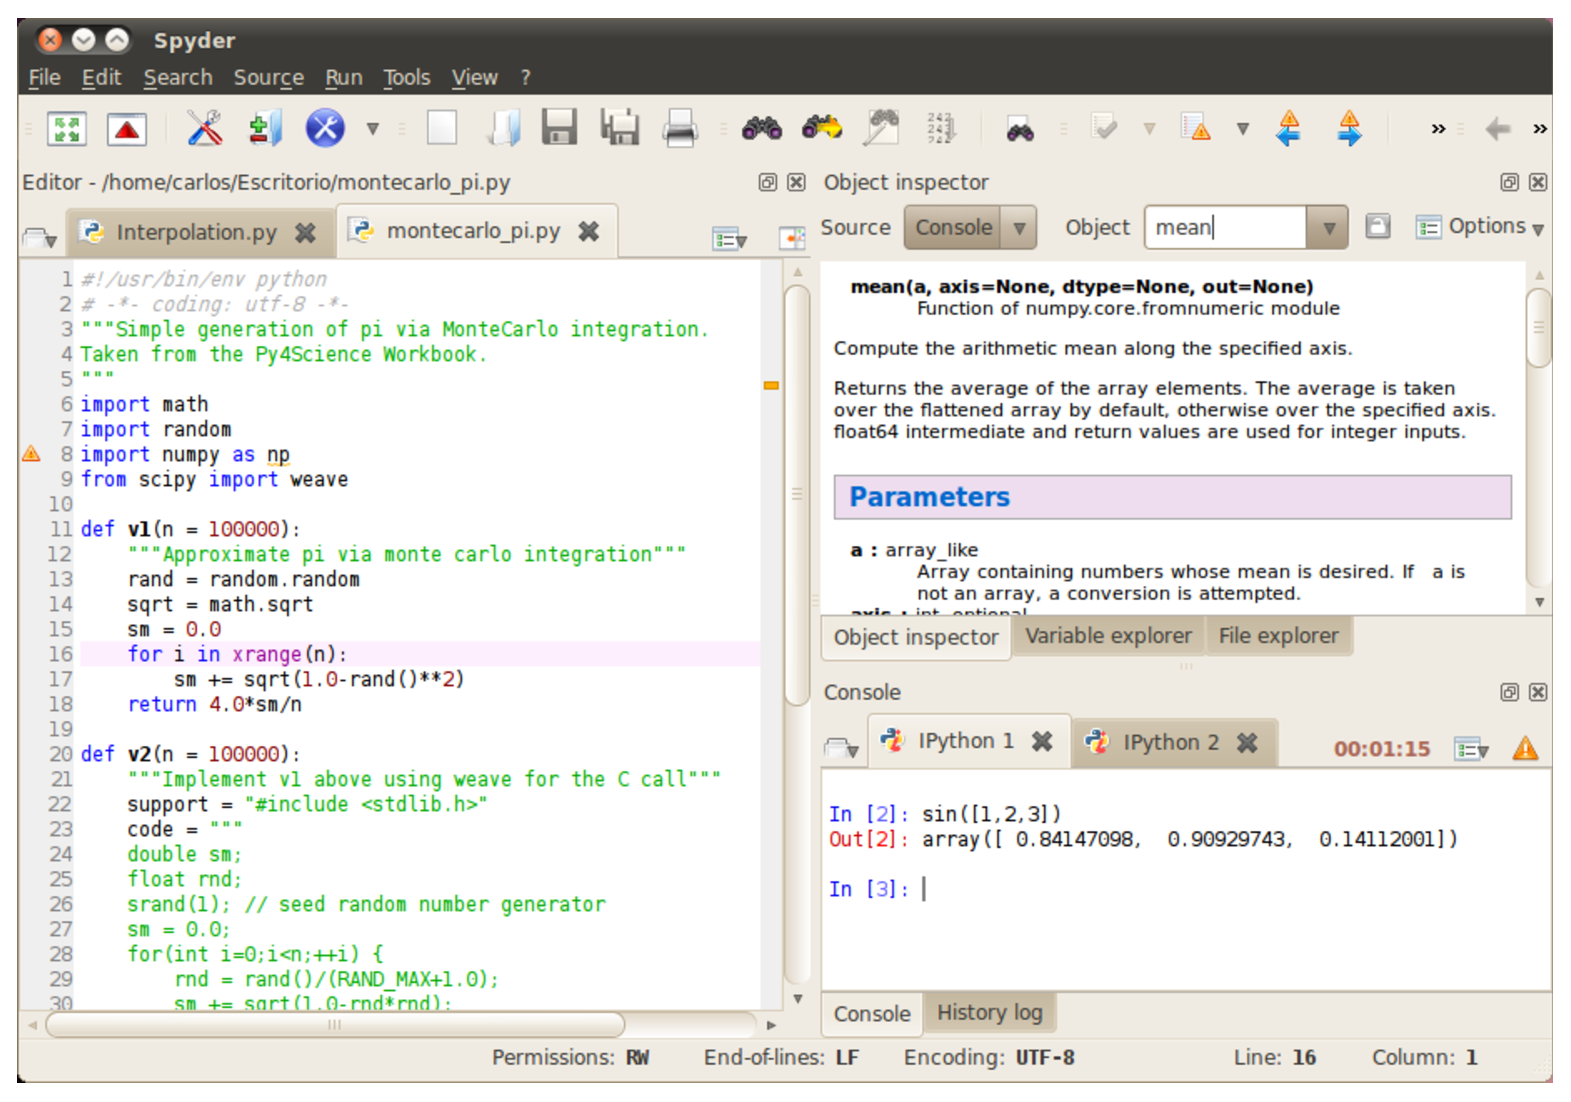
\includegraphics[scale=0.5]{spyder-linux.eps}<2> 
\end{figure}
\end{frame}
\section{Graficaci\'{o}n con Python}
\begin{frame}
\frametitle{Graficaci\'{o}n con Python}
Una buena parte del trabajo que tendremos que hacer como f\'{i}sicos es utilizar un conjunto de datos que por si solos, no van a darnos informaci\'{o}n sobre un modelo o un fen\'{o}meno, por ello, ser\'{a} necesario usar gr\'{a}ficas.
\\
\medskip
Python incluye un m\'{o}dulo de graficaci\'{o}n bastante vers\'{a}til para generar gr\'{a}ficas y exportarlas a diferentes tipos de archivos.
\\
\medskip
La librer\'{i}a se llama \texttt{matplotlib}. Haremos algunos ejercicios para demostrar su potencia.
\end{frame}
\begin{frame}
\texttt{matplotlib.pyplot} es una colecci\'{o}n de funciones de estilo de mando, de tal manera que matplotlib funciona a la manera de MATLAB. Cada instrucci\'{o}n \texttt{pyplot} aplica un cambio a una figura: por ejemplo, crear una figura, crear un \'{a}rea de trazado en una figura, trazar algunas l\'{i}neas en un \'{a}rea de trazado, decorar con etiquetas, etc.
\end{frame}
\begin{frame}[fragile]
\frametitle{Ejecicio 1}
\begin{lstlisting}
import matplotlib.pyplot as plt
plt.plot([1,2,3,4])
plt.ylabel('algunos numeros')
plt.show()
\end{lstlisting}
\begin{figure}
	\centering
	\includegraphics[scale=0.35]{plotEjercicio1.eps}<2> 
\end{figure}
\end{frame}
\begin{frame}
Te estar\'{a}s preguntando por qu\'{e} tenemos en el eje $x$ el rango $0-3$ y en el eje $y$ el rango  $1-4$.
\\
\medskip
Si proporcionamos una \'{u}nica lista o matriz en el comando \texttt{plot}, \texttt{matplotlib} asume que es una secuencia de valores de $y$, por lo que genera autom\'{a}ticamente los valores de $x$ para nosotros. Como los \'{i}ndices en Python comienzan en $0$, el vector $x$ por defecto tiene la misma longitud que $y$, pero inicia con 0. De ah\'{i} que los datos $x$ son $[0,1,2,3]$.
\end{frame}
\begin{frame}[fragile]
\frametitle{Ejecicio 2}
\begin{lstlisting}
import matplotlib.pyplot as plt
plt.plot([1,2,3,4], [1,4,9,16], 'ro')
plt.axis([0, 6, 0, 20])
plt.show()
\end{lstlisting}
\begin{figure}
	\centering
	\includegraphics[scale=0.35]{plotEjercicio2.eps}<2> 
\end{figure}
\end{frame}
\begin{frame}[fragile]
Por cada par $x$, $y$ de argumentos, existe un tercer argumento opcional, que es la cadena de formato que indica el color y tipo de l\'{i}nea.
\\
\medskip
Las letras y los s\'{i}mbolos de la cadena de formato son como en MATLAB, y concatenar una cadena de color con una cadena estilo de l\'{i}nea.
\\
\medskip
La cadena de formato por defecto es \verb|'b-'|, que es una l\'{i}nea de color azul.
\end{frame}
\begin{frame}[fragile]
\begin{tabular}{l | l}
car\'{a}cter & descripci\'{o}n \\ \hline
\verb|'-'|	& l\'{i}nea s\'{o}lida \\ \hline
\verb|'--'| & l\'{i}nea cortada \\ \hline
\verb|'-.'| & l\'{i}nea-punto \\ \hline
\verb|':'|	& l\'{i}nea de puntos \\ \hline
\verb|'.'|	& marca de punto \\ \hline
\verb|','|	& marca de pixel \\ \hline
\verb|'o'|	& marca de c\'{i}rculo \\ \hline
\verb|'v'|	& marca de tri\'{a}ndulo hacia abajo \\ \hline
\verb|'^'|	& marca de tri\'{a}ngulo hacia arriba
\end{tabular}
\end{frame}
\begin{frame}[fragile]
\begin{tabular}{l | l}
car\'{a}cter & color \\ \hline
\verb|'b'| & azul \\ \hline
\verb|'g'| & verde \\ \hline
\verb|'r'| & rojo \\ \hline
\verb|'c'| & cyan \\ \hline
\verb|'m'| & magenta \\ \hline
\verb|'y'| & amarillo \\ \hline
\verb|'k'| & negro \\ \hline
\verb|'w'| & blanco
\end{tabular}
\end{frame}
\begin{frame}
\texttt{matplotlib} se limita a trabajar con listas, por lo que ser\'{i}a bastante acotado para el procesamiento y an\'{a}lisis num\'{e}rico.
\\
\medskip
Por lo general, se utilizan los arreglos del m\'{o}dulo \texttt{numpy}. De hecho, todas las secuencias se convierten en matrices de \texttt{numpy} internamente.
\\
\medskip
El siguiente ejemplo ilustra un trazado de l\'{i}neas con varios estilos diferentes en una sola instucci\'{o}n utilizando arreglos.
\end{frame}
\begin{frame}[fragile]
\frametitle{Ejecicio 3}
\begin{lstlisting}
import numpy as np
import matplotlib.pyplot as plt

t = np.arange(0., 5., 0.2)
plt.plot(t, t, 'r--', t, t**2, 'bs', t, t**3, 'g^')
plt.show()
\end{lstlisting}
\end{frame}
\begin{frame}[fragile]
\begin{figure}
	\centering
	\includegraphics[scale=0.5]{plotEjercicio3.eps}
\end{figure}
\end{frame}
\begin{frame}[fragile]
\frametitle{Ejercicio 4}
Trabajando con m\'{u}ltiples gr\'{a}ficas
\begin{lstlisting}
import numpy as np
import matplotlib.pyplot as plt

def f(t):
    return np.exp(-t) * np.cos(2*np.pi*t)

t1 = np.arange(0.0, 5.0, 0.1)
t2 = np.arange(0.0, 5.0, 0.02)

plt.figure(1)
plt.subplot(211)
plt.plot(t1, f(t1), 'bo', t2, f(t2), 'k')

plt.subplot(212)
plt.plot(t2, np.cos(2*np.pi*t2), 'r--')
\end{lstlisting}
\end{frame}
\begin{frame}[fragile]
\begin{figure}
	\centering
	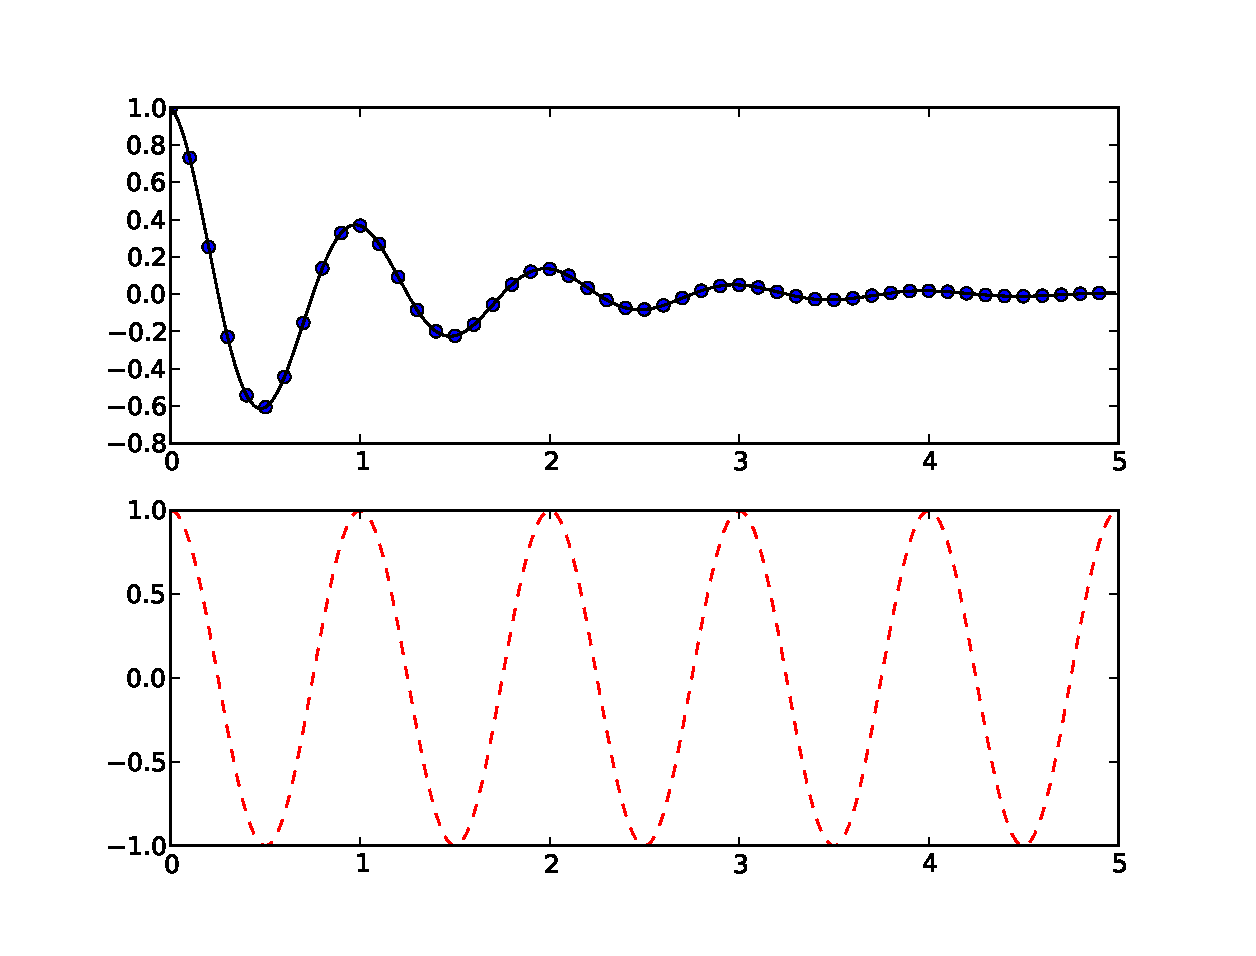
\includegraphics[scale=0.5]{plotEjercicio4.eps}
\end{figure}
\end{frame}
\begin{frame}
El comando \texttt{figure()} aqu\'{i} es opcional, ya \texttt{figure(1)} se crea de forma predeterminada, as\'{i} mismo \texttt{subplot(111)} se crea de forma predeterminada si no se especifica manualmente un eje.
\\
\medskip
El comando \texttt{subplot()} especifica \texttt{numrows, numcols, fignum} donde \texttt{fignum} var\'{i}a en rango de 1 a \texttt{numrows * numcols}. Las comas en el comando \texttt{subplot()} son opcionales si \texttt{numrows * numcols} $<10$. Por tanto \texttt{subplot(211)} es id\'{e}ntica a la \texttt{subplot(2,1,1)}.
\end{frame}
\begin{frame}[fragile]
\frametitle{Ejercicio 5}
\begin{lstlisting}
import matplotlib.pyplot as plt

plt.figure(1)                
plt.subplot(211)         
plt.plot([1,2,3])
plt.subplot(212)         
plt.plot([4,5,6])


plt.figure(2)                
plt.plot([4,5,6])           

plt.figure(1)                
plt.subplot(211)         
plt.title('Tan facil como 1,2,3')
plt.show()
\end{lstlisting}
\end{frame}
\begin{frame}[fragile]
\begin{figure}
	\centering
	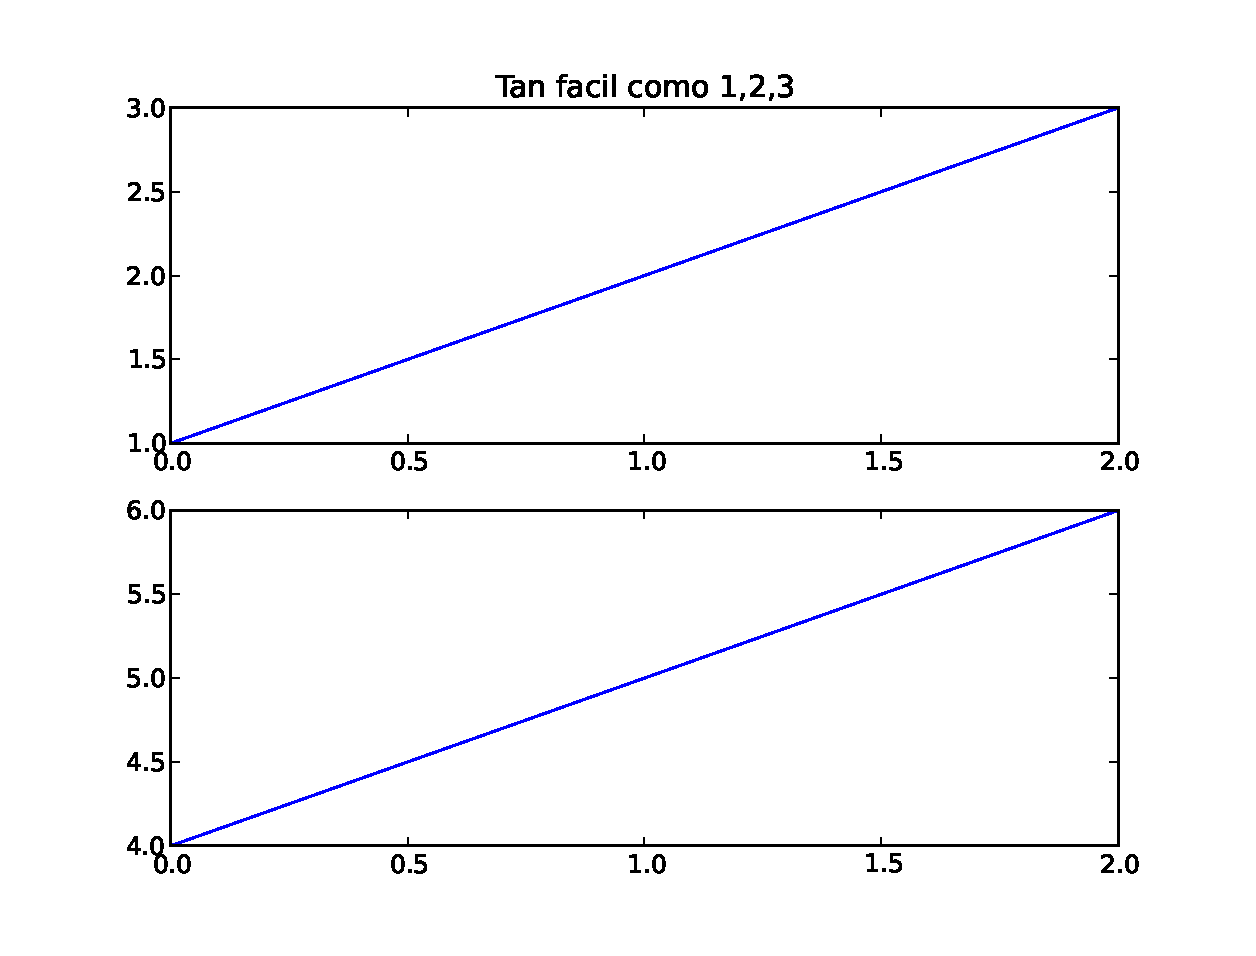
\includegraphics[scale=0.5]{plotEjercicio5_1.eps}<1>
	\includegraphics[scale=0.5]{plotEjercicio5_2.eps}<2>
\end{figure}
\end{frame}
\section{Arreglos}
\begin{frame}
\frametitle{Repaso express sobre arreglos}
Las estructuras de datos que hemos visto hasta ahora permiten manipular datos de manera muy flexible. Combin\'{a}ndolas y anid\'{a}ndolas, es posible organizar informaci\'{o}n de manera estructurada para representar sistemas del mundo real.
\end{frame}
\begin{frame}
En muchas aplicaciones en Ciencias, m\'{a}s importante que la organizaci\'{o}n de los datos es la capacidad de hacer muchas operaciones a la vez sobre grandes conjuntos de datos num\'{e}ricos de manera eficiente. Algunos ejemplos de problemas que requieren manipular grandes secuencias de n\'{u}meros son: la predicción del clima, simulaci\'{o}n, graficaci\'{o}n de modelos, la construcci\'{o}n de edificios, y el an\'{a}lisis de indicadores financieros entre muchos otros.
\end{frame}
\begin{frame}
La estructura de datos que sirve para almacenar estas grandes secuencias de n\'{u}meros (generalmente de tipo float) es el \textbf{arreglo}.
\\
\bigskip
Los arreglos tienen algunas similitudes con las listas:
\begin{itemize}
\item los elementos tienen un orden y se pueden acceder mediante su posici\'{o}n.
\item los elementos se pueden recorrer usando un ciclo \texttt{for}.
\end{itemize}
\end{frame}
\begin{frame}
Sin embargo, tambi\'{e}n tienen algunas restricciones:
\begin{itemize}
\item todos los elementos del arreglo deben tener el mismo tipo.
\item en general, el tamaño del arreglo es fijo (no van creciendo din\'{a}micamente como las listas).
\item se ocupan principalmente para almacenar datos num\'{e}ricos.
\end{itemize}
\end{frame}
\begin{frame}
Los arreglos son los equivalentes en programaci\'{o}n de las matrices y vectores en matem\'{a}ticas. Precisamente, una gran motivaci\'{o}n para usar arreglos es que hay mucha teor\'{i}a detr\'{a}s de ellos que puede ser usada en el diseño de algoritmos para resolver problemas verdaderamente interesantes.
\end{frame}
\subsection{Crear arreglos}
\begin{frame}[fragile]
\frametitle{Crear arreglos}
El m\'{o}dulo que provee las estructuras de datos y las funciones para trabajar con arreglos es \texttt{NumPy}.
\begin{verbatim}
from numpy import array
\end{verbatim}
Como estaremos usando frecuentemente muchas funciones de este m\'{o}dulo, conviene importarlas todas de una vez usando la siguiente sentencia:
\begin{verbatim}
from numpy import *
\end{verbatim}
\end{frame}
\begin{frame}[fragile]
El tipo de datos de los arreglos se llama \textcolor{blue}{array}. Para crear un arreglo nuevo, se puede usar la funci\'{o}n array pas\'{a}ndole como par\'{a}metro la lista de valores que deseamos agregar al arreglo:
\begin{exampleblock}{}<2->
\pause
\verb|>>> a = array([6, 1, 3, 9, 8])| \\
\pause
\verb|>>> a|  \\
\pause
\verb|array([6, 1, 3, 9, 8])|
\end{exampleblock}
\pause
Todos los elementos del arreglo tienen exactamente el mismo tipo. Para crear un arreglo de n\'{u}meros reales, basta con que uno de los valores lo sea:
\pause
\begin{exampleblock}{}<3->
\pause
\verb|>>> b = array([6.0, 1, 3, 9, 8])| \\
\pause
\verb|>>> b| \\
\pause
\verb|array([ 6.,  1.,  3.,  9.,  8.])| 
\end{exampleblock}
\end{frame}
\begin{frame}[fragile]
Otra opci\'{o}n es convertir el arreglo a otro tipo usando el m\'{e}todo \texttt{astype:}
\begin{exampleblock}{}<2->
\verb|>>> a| \\
\pause
\verb|array([6, 1, 3, 9, 8])| \\
\pause
\verb|>>> a.astype(float)| \\
\pause
\verb|array([ 6.,  1.,  3.,  9.,  8.])| \\
\pause
\verb|>>> a.astype(complex)| \\
\pause
\verb|array([ 6.+0.j,  1.+0.j,  3.+0.j,  9.+0.j,  8.+0.j])|
\end{exampleblock}
\end{frame}
\begin{frame}[fragile]
Hay muchas formas de arreglos que aparecen a menudo en la pr\'{a}ctica, por lo que existen funciones especiales para crearlos:
\begin{itemize}[<+->]
\item \texttt{zeros(n)} crea un arreglo de $n$ ceros.
\item \texttt{ones(n)} crea un arreglo de $n$ unos.
\item \texttt{arange(a, b, c)} crea un arreglo de forma similar a la funci\'{o}n \texttt{range}, con las diferencias que $a$, $b$ y $c$ pueden ser reales, y que el resultado es un arreglo y no una lista.
\item \texttt{linspace(a, b, n)} crea un arreglo de $n$ valores equiespaciados entre $a$ y $b$.
\end{itemize}
\end{frame}
\begin{frame}[fragile]
\begin{exampleblock}{}<2->
\verb|>>> zeros(6)| \\
\pause
\verb|array([ 0.,  0.,  0.,  0.,  0.,  0.])|
\pause
\verb|>>> ones(5)| \\
\pause
\verb|array([ 1.,  1.,  1.,  1.,  1.])| \\
\pause
\verb|>>> arange(3.0, 9.0)| \\
\pause
\verb|array([ 3.,  4.,  5.,  6.,  7.,  8.])|\\
\pause
\verb|>>> linspace(1, 2, 5)| \\
\pause
\verb|array([ 1.  ,  1.25,  1.5 ,  1.75,  2.  ])|
\end{exampleblock}
\end{frame}
\subsection{Operaciones con arreglos}
\begin{frame}[fragile]
\frametitle{Operaciones con arreglos}
Las limitaciones que tienen los arreglos respecto de las listas son compensadas por la cantidad de operaciones convenientes que permiten realizar sobre ellos.
\\
\bigskip
Las operaciones aritm\'{e}ticas entre arreglos se aplican elemento a elemento:
\fontsize{12}{12}\selectfont
\begin{exampleblock}{}
\verb|>>> a = array([55, 21, 19, 11,  9])|
\verb|>>> b = array([12, -9,  0, 22, -9])|
\end{exampleblock}
\begin{exampleblock}{sumar los dos arreglos elemento a elemento}<2->
\verb|>>> a + b| \\
\verb|array([67, 12, 19, 33,  0])|
\end{exampleblock}
\end{frame}
\begin{frame}[fragile]
\begin{exampleblock}{multiplicar por $0.1$ todos los elementos}
\verb|>>> 0.1 * a| \\
\verb|array([ 5.5,  2.1,  1.9,  1.1,  0.9])|
\end{exampleblock}
\begin{exampleblock}{restar $9.0$ a todos los elementos}<2->
\verb|>>> a - 9.0| \\
\verb|array([ 46.,  12.,  10.,   2.,   0.])|
\end{exampleblock}
Note que si quisi\'{e}ramos hacer estas operaciones usando listas, necesitar\'{i}amos usar un ciclo para hacer las operaciones elemento a elemento.
\end{frame}
\begin{frame}[fragile]
Las operaciones relacionales tambi\'{e}n se aplican elemento a elemento, y devuelven un arreglo de valores booleanos:
\fontsize{12}{12}\selectfont
\begin{exampleblock}{}<2->
\verb|>>> a = array([5.1, 2.4, 3.8, 3.9])| \\
\verb|>>> b = array([4.2, 8.7, 3.9, 0.3])| \\
\verb|>>> c = array([5, 2, 4, 4]) + array([1, 4, -2, -1])/10.0|\\
\pause
\verb|>>> a < b| \\
\pause
\verb|array([False,  True,  True, False], dtype=bool)| \\
\pause
\verb|>>> a == c| \\
\pause
\verb|array([ True,  True,  True,  True], dtype=bool)|
\end{exampleblock}
\end{frame}
\begin{frame}[fragile]
Para reducir el arreglo de booleanos a un \'{u}nico valor, se puede usar las funciones \texttt{any} y \texttt{all.any} devuelve \texttt{True} si al menos uno de los elementos es verdadero, mientras que \texttt{all} devuelve \texttt{True} s\'{o}lo si todos lo son (del ingl\'{e}s, \texttt{any} signfica \textit{alguno}, y \texttt{all} significa \textit{todos}):
\begin{exampleblock}{}<2->
\verb|>>> any(a < b)| \\
\pause
\verb|True| \\
\pause
\verb|>>> any(a == b)| \\
\pause
\verb|False| \\
\pause
\verb|>>> all(a == c)| \\
\pause
\verb|True|
\end{exampleblock}
\end{frame}
\subsection{Funciones sobre arreglos}
\begin{frame}[fragile]
\frametitle{Funciones sobre arreglos}
\texttt{NumPy} provee muchas funciones matem\'{a}ticas que tambi\'{e}n operan elemento a elemento.
\begin{exampleblock}{}<2->
\verb|>>> from numpy import linspace, pi, sin| \\
\verb|>>> x = linspace(0, pi/2, 9)| \\
\fontsize{10}{10}\selectfont
\verb|>>> x| \\
\pause
\verb|array([ 0.        ,  0.19634954,  0.39269908,|\\ 
\verb|        0.58904862,  0.78539816,  0.9817477 ,|\\
\verb|        1.17809725,  1.37444679,  1.57079633])| \\
\verb|>>> sin(x)| \\
\pause
\verb|array([ 0.        ,  0.19509032,  0.38268343,| \\
\verb|        0.55557023,  0.70710678,  0.83146961,| \\
\verb|        0.92387953,  0.98078528,  1.        ])|
\end{exampleblock}
Como puede ver, los valores obtenidos van de 0 a 1, que es justamente como se comporta la función seno en el intervalo $[0, \pi/2]$.
\end{frame}
\begin{frame}[fragile]
Aqu\'{i} tambi\'{e}n se hace evidente otra de las ventajas de los arreglos: al mostrarlos en la consola o al imprimirlos, los valores aparecen perfectamente alineados. Con las listas, esto no ocurre:
\fontsize{12}{12}\selectfont
\begin{exampleblock}{}
\verb|>>> list(sin(x))| \\
\pause
\verb|[0.0, 0.19509032201612825, 0.38268343236508978, 0.5555702330| \\
\verb|1960218, 0.70710678118654746, 0.83146961230254524, 0.9238795| \\
\verb|3251128674, 0.98078528040323043, 1.0]|
\end{exampleblock}
\end{frame}
\subsection{Arreglos aleatorios}
\begin{frame}[fragile]
\frametitle{Arreglos aleatorios}
\texttt{NumPy} contiene a su vez otros m\'{o}dulos que proveen funcionalidad adicional a los arreglos y funciones b\'{a}sicos.
\\
\bigskip
El m\'{o}dulo \texttt{numpy.random} provee funciones para crear n\'{u}meros aleatorios (es decir, generados al azar), de las cuales la m\'{a}s usada es la funci\'{o}n \texttt{random}, que entrega un arreglo de n\'{u}meros al azar distribuidos uniformemente entre 0 y 1:
\\
\bigskip
\verb|>>> from numpy.random import random|
\end{frame}
\begin{frame}[fragile]
\fontsize{12}{12}\selectfont
\begin{exampleblock}{}
\verb|>>> random(3)| \\
\pause
\verb|array([ 0.53077263,  0.22039319,  0.81268786])| \\
\verb|>>> random(3)| \\
\pause
\verb|array([ 0.07405763,  0.04083838,  0.72962968])| \\
\pause
\verb|>>> random(3)| \\
\pause
\verb|array([ 0.51886706,  0.46220545,  0.95818726])|
\end{exampleblock}
\end{frame}
\subsection{Obtener elementos de un arreglo}
\begin{frame}[fragile]
\frametitle{Obtener elementos de un arreglo}
Cada elemento del arreglo tiene un \'{i}ndice, al igual que en las listas. El primer elemento tiene \'{i}ndice $0$. Los elementos tambi\'{e}n pueden numerarse desde el final hasta el principio usando \'{i}ndices negativos. El \'{u}ltimo elemento tiene \'{i}ndice $-1$:
\fontsize{12}{12}\selectfont
\begin{exampleblock}{}<2->
\verb|>>> a = array([6.2, -2.3, 3.4, 4.7, 9.8])| \\
\pause
\verb|>>> a[0]| \\
\pause
\verb|6.2| \\
\pause
\verb|>>> a[1]| \\
\pause
\verb|-2.3| \\
\pause
\verb|>>> a[-2]| \\
\pause
\verb|4.7| \\
\pause
\verb|>>> a[3]| \\
\pause
\verb|4.7|
\end{exampleblock}
\end{frame}
\begin{frame}[fragile]
Una secci\'{o}n del arreglo puede ser obtenida usando el operador de rebanado $a[i:j]$. Los \'{i}ndices $i$ y $j$ indican el rango de valores que ser\'{a}n devueltos:
\begin{exampleblock}{}<2->
\verb|>>> a| \\
\pause
\verb|array([ 6.2, -2.3,  3.4,  4.7,  9.8])| \\
\pause
\verb|>>> a[1:4]| \\
\pause
\verb|array([-2.3,  3.4,  4.7])| \\
\pause
\verb|>>> a[2:-2]| \\
\pause
\verb|array([ 3.4])|
\end{exampleblock}
\end{frame}
\begin{frame}[fragile]
Si el primer \'{i}ndice es omitido, el rebanado comienza desde el principio del arreglo. Si el segundo \'{i}ndice es omitido, el rebanado termina al final del arreglo:
\begin{exampleblock}{}<2->
\verb|>>> a[:2]| \\
\pause
\verb|array([ 6.2, -2.3])| \\
\pause
\verb|>>> a[2:]| \\
\pause
\verb|array([ 3.4,  4.7,  9.8])|
\end{exampleblock}
\end{frame}
\begin{frame}[fragile]
Un tercer \'{i}ndice puede indicar cada cu\'{a}ntos elementos ser\'{a}n incluidos en el resultado:
\fontsize{12}{12}\selectfont
\begin{exampleblock}{}<2->
\verb|>>> a = linspace(0, 1, 9)| \\
\pause
\verb|>>> a| \\
\pause
\verb|array([ 0.   ,  0.125,  0.25 ,  0.375,  0.5  ,  0.625,  0.75 ,  0.875,  1.   ])| \\
\pause
\verb|>>> a[1:7:2]| \\
\pause
\verb|array([ 0.125,  0.375,  0.625])| \\
\pause
\verb|>>> a[::3]| \\
\pause
\verb|array([ 0.   ,  0.375,  0.75 ])| \\
\pause
\verb|>>> a[-2::-2]| \\
\pause
\verb|array([ 0.875,  0.625,  0.375,  0.125])| \\
\pause
\verb|>>> a[::-1]| \\
\pause
\verb|array([ 1.   ,  0.875,  0.75 ,  0.625,  0.5  ,  0.375,  0.25 ,  0.125,  0.   ])|
\end{exampleblock}
\end{frame}
\begin{frame}[fragile]
Una manera simple de recordar c\'{o}mo funciona el rebanado es considerar que los \'{i}ndices no se refieren a los elementos, sino a los espacios entre los elementos:
\fontsize{12}{12}\selectfont
\begin{exampleblock}{}<2->
\verb|>>> b = array([17.41, 2.19, 10.99, -2.29, 3.86, 11.10])| \\
\pause
\verb|>>> b[2:5]| \\
\pause
\verb|array([ 10.99,  -2.29,   3.86])| \\
\pause
\verb|>>> b[:5]| \\
\pause
\verb|array([ 17.41,   2.19,  10.99,  -2.29,   3.86])| \\
\pause
\verb|>>> b[1:1]| \\
\pause
\verb|array([], dtype=float64)| \\
\pause
\verb|>>> b[1:5:2]| \\
\pause
\verb|array([ 2.19, -2.29])|
\end{exampleblock}
\end{frame}
\subsection{Algunos m\'{e}todos convenientes}
\begin{frame}[fragile]
\frametitle{Algunos m\'{e}todos convenientes}
Los arreglos proveen algunos m\'{e}todos \'{u}tiles que conviene conocer.
\\
\bigskip
Los m\'{e}todos \texttt{min} y \texttt{max}, entregan respectivamente el m\'{i}nimo y el m\'{a}ximo de los elementos del arreglo:
\begin{exampleblock}{}<2->
\verb|>>> a = array([4.1, 2.7, 8.4, pi, -2.5, 3, 5.2])| \\
\pause
\verb|>>> a.min()| \\
\pause
\verb|-2.5| \\
\pause
\verb|>>> a.max()| \\
\pause
\verb|8.4000000000000004|
\end{exampleblock}
\end{frame}
\begin{frame}[fragile]
Los m\'{e}todos \texttt{argmin} y \texttt{argmax} entregan respectivamente la posici\'{o}n del m\'{i}nimo y del m\'{a}ximo:
\begin{exampleblock}{}<2->
\verb|>>> a.argmin()| \\
\pause
\verb|4| \\
\pause
\verb|>>> a.argmax()| \\
\pause
\verb|2|
\end{exampleblock}
\end{frame}
\begin{frame}[fragile]
Los m\'{e}todos \texttt{sum} y \texttt{prod} entregan respectivamente la suma y el producto de los elementos:
\begin{exampleblock}{}<2->
\verb|>>> a.sum()| \\
\pause
\verb|24.041592653589795| \\
\pause
\verb|>>> a.prod()| \\
\pause
\verb|-11393.086289208301|
\end{exampleblock}
\end{frame}
\subsection{Productos entre arreglos}
\begin{frame}
\frametitle{Productos entre arreglos}
Recordemos que vector es sin\'{o}nimo de arreglo de una dimensi\'{o}n, y matriz es sin\'{o}nimo de arreglo de dos dimensiones.
\end{frame}
\subsubsection{Producto interno (vector-vector)}
\begin{frame}[fragile]
\frametitle{Producto interno (vector-vector)}
El producto interno entre dos vectores se obtiene usando la funci\'{o}n \texttt{dot} provista por NumPy:
\fontsize{12}{12}\selectfont
\begin{exampleblock}{}
\verb|>>> a = array([-2.8 , -0.88,  2.76,  1.3 ,  4.43])| \\
\verb|>>> b = array([ 0.25, -1.58,  1.32, -0.34, -4.22])| \\
\pause
\verb|>>> dot(a, b)| \\
\pause
\verb|-14.803|
\end{exampleblock}
\end{frame}
\begin{frame}[fragile]
El producto interno es una operaci\'{o}n muy com\'{u}n. Por ejemplo, suele usarse para calcular totales:
\fontsize{12}{12}\selectfont
\begin{exampleblock}{}
\verb|>>> precios = array([200, 100, 500, 400, 400, 150])|
\verb|>>> cantidades = array([1, 0, 0, 2, 1, 0])|
\pause
\verb|>>> total_a_pagar = dot(precios, cantidades)|
\pause
\verb|>>> total_a_pagar|
\pause
\verb|1400|
\end{exampleblock}
Tambi\'{e}n se usa para calcular promedios ponderados:
\begin{exampleblock}{}
\verb|>>> notas = array([45, 98, 32])| \\
\pause
\verb|>>> ponderaciones = array([30, 30, 40]) / 100.| \\
\pause
\verb|>>> nota_final = dot(notas, ponderaciones)| \\
\pause
\verb|>>> nota_final| \\
\verb|55.7|
\end{exampleblock}
\end{frame}
\subsubsection{Producto matriz-vector}
\begin{frame}[fragile]
\frametitle{Producto matriz-vector}
El producto matriz-vector es el vector de los productos internos. El producto matriz-vector puede ser visto simplemente como varios productos internos calculados de una sola vez.
\\
\bigskip
Esta operaci\'{o}n tambi\'{e}n es obtenida usando la funci\'{o}n \texttt{dot} entre las filas de la matriz y el vector:
\fontsize{12}{12}\selectfont
\begin{exampleblock}{}
\verb|>>> a = array([[-0.6,  4.8, -1.2],| \\
\verb|               [-2. , -3.6, -2.1],| \\
\verb|               [ 1.7,  4.9,  0. ]])| \\
\verb|>>> x = array([-0.6, -2. ,  1.7])| \\
\pause
\verb|>>> dot(a, x)| \\
\pause
\verb|array([-11.28,   4.83, -10.82])|
\end{exampleblock}
\end{frame}
\subsubsection{Producto matriz-matriz}
\begin{frame}[fragile]
\frametitle{Producto matriz-matriz}
\fontsize{12}{12}\selectfont
El producto matriz-matriz es la matriz de los productos internos entre las filas de la primera matriz y las columnas de la segunda.
\begin{exampleblock}{}
\verb|>>> a = array([[ 2,  8],| \\
\verb|               [-3,  7],| \\
\verb|               [-8, -5]])| \\
\verb|>>> b array([[-3, -5, -6, -3],| \\
\verb|             [-9, -2,  3, -3]])| \\
\pause
\verb|>>> dot(a, b)| \\
\pause
\verb|array([[-78, -26,  12, -30],|\\
\verb|       [-54,   1,  39, -12],| \\
\verb|       [ 69,  50,  33,  39]])| \\
\end{exampleblock}
\end{frame}
\begin{frame}
La multiplicaci\'{o}n de matrices puede ser vista como varios productos matriz-vector (usando como vectores todas las filas de la segunda matriz), calculados de una sola vez.
\end{frame}
\begin{frame}
En resumen, al usar la función \texttt{dot}, la estructura del resultado depende de cu\'{a}les son los par\'{a}metros pasados:
\begin{enumerate}[<+->]
\item \texttt{dot}(vector, vector) $\rightarrow$ n\'{u}mero.
\item \texttt{dot}(matriz, vector) $\rightarrow$ vector.
\item \texttt{dot}(matriz, matriz) $\rightarrow$ matriz.
\end{enumerate}
\end{frame}
\section{Soluci\'{o}n de sistemas de ecuaciones}
\begin{frame}
\frametitle{Soluci\'{o}n de sistemas lineales}
\fontsize{12}{12}\selectfont
Un problema recurrente en Ciencias consiste en obtener cu\'{a}l es el vector x cuando A y b son dados:
\[Ax=b\]
La ecuaci\'{o}n matricial $Ax=b$ es una manera abreviada de expresar un sistema de ecuaciones lineales. Por ejemplo, la ecuaci\'{o}n del diagrama es equivalente al siguiente sistema de tres ecuaciones que tiene las tres inc\'{o}gnitas $w$, $y$ y $z$:
\begin{eqnarray*}
36w+51y+13z &=& 3 \\
52w+34y+74z &=& 45 \\
7y+1.1z &=& 33
\end{eqnarray*}
\end{frame}
\begin{frame}
Este sistema se representa matricialmente:
\[ \begin{bmatrix}
36 & 51 & 13 \\
52 & 34 & 74 \\
 & 7 &1.1
\end{bmatrix}
\begin{bmatrix}
w \\
y \\
z
\end{bmatrix} =
\begin{bmatrix}
3 \\
45 \\
33
\end{bmatrix}
\]
\end{frame}
\begin{frame}[fragile]
La teor\'{i}a detr\'{a}s de la soluci\'{o}n de problemas de este tipo, se puede consultar en cualquier texto de \'{a}lgebra lineal. Sin embargo, como este tipo de problemas aparece a menudo en la pr\'{a}ctica, aprenderemos c\'{o}mo obtener r\'{a}pidamente la soluci\'{o}n usando Python.
\\
\bigskip
Dentro de los varios m\'{o}dulos incluidos en NumPy, est\'{a} el m\'{o}dulo \texttt{numpy.linalg}, que provee algunas funciones que implementan algoritmos de \'{a}lgebra lineal. Dentro de este m\'{o}dulo est\'{a} la funci\'{o}n \texttt{solve}, que entrega la solución $x$ de un sistema a partir de la matriz $A$ y el vector $b$:
\end{frame}
\begin{frame}[fragile]
\fontsize{12}{12}\selectfont
\begin{exampleblock}{}
\verb|>>> a = array([[ 36. ,  51. ,  13. ],| \\
\verb|...            [ 52. ,  34. ,  74. ],| \\
\verb|...            [  0. ,   7. ,   1.1]])| \\
\pause
\verb|>>> b = array([  3.,  45.,  33.])| \\
\pause
\verb|>>> x = solve(a, b)| \\
\pause
\verb|>>> x| \\
\pause
\verb|array([-7.10829222,  4.13213834,  3.70457422])|
\end{exampleblock}
Podemos ver que el vector $x$ en efecto satisface la ecuaci\'{o}n $Ax = b$:
\begin{exampleblock}{}
\verb|>>> dot(a, x)| \\
\pause
\verb|array([  3.,  45.,  33.])| \\
\pause
\verb|>>> b| \\
\pause
\verb|array([  3.,  45.,  33.])|
\end{exampleblock}
\end{frame}
\begin{frame}[fragile]
Sin embargo, es importante tener en cuenta que los valores de tipo real casi nunca est\'{a}n representados de manera exacta en la soluci\'{o}n num\'{e}rica, y que el resultado de un algoritmo que involucra muchas operaciones puede sufrir de algunos errores de redondeo. Por esto mismo, puede ocurrir que aunque los resultados se vean iguales en la consola, los datos obtenidos son s\'{o}lo aproximaciones y no exactamente los mismos valores:
\begin{exampleblock}{}
\verb|>>> (dot(a, x) == b).all()| \\
\pause
\verb|False|
\end{exampleblock}
\end{frame}
\section{Otras funciones dentro de \texttt{numpy.linalg}}
\begin{frame}
\frametitle{Otras funciones dentro de \texttt{numpy.linalg}}
Para extender (y simplificar el trabajo para codificar) el manejo de arreglos en Python, se cuenta con otras funciones que se ocupan de manera continua.
\\
\bigskip
Como se ha mencionado anteriormente, es necesario repasar el \'{a}lgebra lineal b\'{a}sica para tener en cuenta el proceso con el cual, Pyhon devuelve una respuesta.
\end{frame}
\subsection{Funci\'{o}n \texttt{Eye}}
\begin{frame}[fragile]
\frametitle{Funci\'{o}n \texttt{Eye}}
La funci\'{o}n \texttt{eye} genera una matriz $N \times	N$ diagonal con \verb|eye(N)|, pero admite otros par\'{a}metros que permiten hacer matrices no cuadradas, tener otro tipo de datos y hacer distinto de $0$ otra diagonal diferente.
\begin{exampleblock}{}
\verb|>>>eye(2)| \\
\pause
\verb|array([[ 1.,  0.],| \\
\verb|       [ 0.,  1.]])|
\end{exampleblock}
\end{frame}
\begin{frame}[fragile]
\begin{exampleblock}{}
\verb|>>> eye(2,3)| \\
\pause
\pause{\verb|array([[ 1.,  0.,  0.],| \\
\verb|       [ 0.,  1.,  0.]])|}
\end{exampleblock}
\begin{exampleblock}{}<2->
\verb|>>> eye(2,3,k=1)| \\
\pause{\verb|array([[ 0.,  1.,  0.],| \\
\verb|       [ 0.,  0.,  1.]])|}
\end{exampleblock}
\begin{exampleblock}{}<3->
\verb|>>> eye(2,3,k=1,dtype=complex)| \\
\pause{\verb|array([[ 0.+0.j,  1.+0.j,  0.+0.j],| \\
\verb|       [ 0.+0.j,  0.+0.j,  1.+0.j]])|}
\end{exampleblock}
\end{frame}
\subsection{Funci\'{o}n \texttt{reshape}}
\begin{frame}
\frametitle{Funci\'{o}n \texttt{reshape}}
La funci\'{o}n \texttt{reshape} permite cambiar las dimensiones de una matriz, siempre respetando el n\'{u}mero total de elementos.
\\
\bigskip
No cambia el objeto original, pero devuelve otro objeto que apunta los mismos datos, de forma que si modificamos uno, el otro lo har\'{a} tambi\'{e}n.
\end{frame}
\begin{frame}[fragile]
\verb|>>> a = random.rand(4,4)| \\
\fontsize{10}{10}\selectfont
\pause
\verb|>>> a| \\
\verb|array([[ 0.51878337,  0.93337481,  0.84368137,  0.07324918],| \\
\verb|       [ 0.12929511,  0.92344357,  0.50366378,  0.59754141],| \\
\verb|       [ 0.67841199,  0.73959186,  0.45789404,  0.85003645],| \\
\verb|       [ 0.95552903,  0.81794353,  0.78810869,  0.05192744]])|
\end{frame}
\begin{frame}[fragile]
\verb|>>> b = reshape(a,(2,8))| \\
\fontsize{10}{10}\selectfont
\pause
\verb|>>> b| \\
\pause
\verb|array([[ 0.51878337,  0.93337481,  0.84368137,  0.07324918,  0.12929511,| \\
\verb|         0.92344357,  0.50366378,  0.59754141],| \\
\verb|       [ 0.67841199,  0.73959186,  0.45789404,  0.85003645,  0.95552903,| \\
\verb|         0.81794353,  0.78810869,  0.05192744]])|
\end{frame}
\subsection{Traza y determinante}
\begin{frame}[fragile]
\frametitle{Traza y determinante}
La traza y el determinante de una matriz, se pueden obtener respectivamente, con la funci\'{o}n \texttt{trace} y \texttt{det}:
\begin{exampleblock}{}
\verb|>>> linalg.det(eye(3))| \\
\pause{\verb|1.0|} \\
\pause{\verb|>>> trace(eye(3))|} \\
\pause{\verb|3.0|}
\end{exampleblock}
\end{frame}
\subsection{Inversa de una matriz}
\begin{frame}[fragile]
\frametitle{Inversa de una matriz}
La inversa de una matriz se calcula con la funci\'{o}n \texttt{inv}:
\begin{exampleblock}{}
\fontsize{12}{12}\selectfont
\verb|>>> a = random.rand(2,2)| \\
\pause{\verb|>>> a|} \\
\pause{\verb|array([[ 0.64569289,  0.72496086],| \\
\verb|       [ 0.98555394,  0.02864243]])| }\\
\pause{\verb|>>> linalg.inv(a)|} \\
\pause{\verb|array([[-0.04115328,  1.04161968],| \\
\verb|       [ 1.41603835, -0.92772791]])|} \\
\pause{\verb|>>> dot(a,linalg.inv(a))|} \\
\pause{\verb|array([[ 1.,  0.],| \\
\verb|       [ 0.,  1.]])|}
\end{exampleblock}
\end{frame}
\subsection{Matriz transpuesta}
\begin{frame}[fragile]
\frametitle{Matriz transpuesta}
La transpuesta de una matriz se obtiene con \texttt{tranpose}, que puede usarse tambi\'{e}n como m\'{e}todo. Otra manera es usar el atributo \texttt{.T}
\begin{exampleblock}{Como funci\'{o}n}
\verb|>>> transpose(a)| \\
\pause{\verb|array([[ 0.64569289,  0.98555394],| \\
\verb|       [ 0.72496086,  0.02864243]])|}
\end{exampleblock}
\end{frame}
\begin{frame}[fragile]
\begin{exampleblock}{Como m\'{e}todo}
\verb|>>> a.transpose()| \\
\pause{\verb|array([[ 0.64569289,  0.98555394],| \\
\verb|       [ 0.72496086,  0.02864243]])|}
\end{exampleblock}
\begin{exampleblock}{Con el atributo \texttt{.T}}<2->
\verb|>>> a.T| \\
\pause{\verb|array([[ 0.64569289,  0.98555394],| \\
\verb|       [ 0.72496086,  0.02864243]])|}
\end{exampleblock}
\end{frame}
\subsection{Valores y vectores propios}
\begin{frame}[fragile]
\frametitle{Valores y vectores propios}
La funci\'{o}n \texttt{eig} permite obtener los valores y vectores propios:
\begin{exampleblock}{}
\verb|>>> linalg.eig(a)| \\
\verb|(array([ 1.23698756, -0.56265224]),| \\
\verb| array([[ 0.77492825, -0.51447164],| \\
\verb|       [ 0.63204921,  0.85750739]]))|
\end{exampleblock}
\end{frame}
\end{document}
